\documentclass[t,xcolor={svgnames,table}]{beamer}

\mode<presentation>
\usetheme{Warsaw}
\useoutertheme{infolines} 

\usepackage{lmodern}
\usepackage{amsmath}
\usepackage{amsfonts}
\usepackage{bbm}
\usepackage{bm}
\usepackage{nicefrac}
\usepackage{color}
\usepackage{multirow}
\usepackage{multicol}
\usepackage{adjustbox}
\usepackage{tikz}
\usepackage{tikz-dependency}
\usepackage{tikz-qtree}
\usepackage{pgfplots,pgfplotstable}
\usepackage{pgf}
\usepackage{collcell}
\usepackage{booktabs}
\usepackage{soul}

% Outline slides
\AtBeginSection[]
{\begin{frame} \frametitle{Outline} \tableofcontents[currentsection,currentsubsection] \end{frame}}


\begin{document}


\title[]{The Language of Legal and Illegal Activity \\ on the Darknet}
\author[Daniel Hershcovich]{Leshem Choshen, Dan Eldad, \textbf{Daniel Hershcovich}, \\
Elior Sulem and Omri Abend }
\date[]{ACL 2019 \\
	\hspace{0.5cm}

\includegraphics[width=.5\textwidth]{huji_banner.png}

\includegraphics[width=.1\textwidth]{huji_logo.jpg}}

\begin{frame}
\titlepage
\end{frame}

\section*{Introduction}

{\usebackgroundtemplate{
	\vbox to \paperheight{\vfil\hbox to \paperwidth{\hfil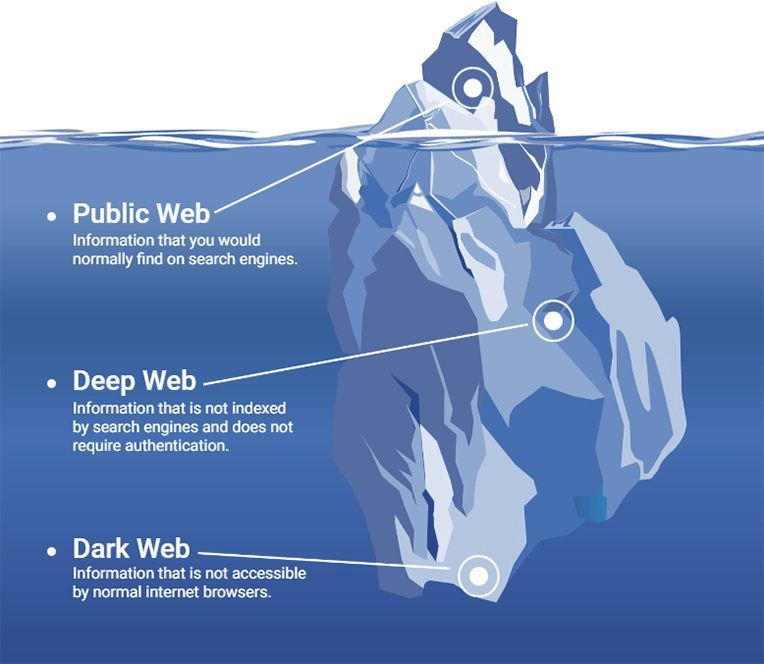
\includegraphics[width=.92\paperwidth]{DarkNet}\hfil}}	
	}%
\begin{frame}
	What is the Dark Web (Darknet)?
	% TODO: examples
\end{frame}
}

\section{Data: Darknet \& eBay}

\begin{frame}
	\frametitle{Data - existing and gathered}
	\begin{itemize}
		\item DUTA-10K, illegal vs. legal drugs \cite{AlNabki19}.
		DUTA-10K contains 10367 websites (Hidden Services).
		20\% are illegal and 48\% are legal (32\% unavailable).
		Illegal drugs are 23\% of illegal websites.
		\item Manually acquired eBay products of drugs weed etc.
	\end{itemize}
\end{frame}

\begin{frame}
	\frametitle{Cleaning}
	% TODO
\end{frame}

\section{Domain Differences: Vocabulary \& Named Entities}

\begin{frame}
	\frametitle{Vocabulary}
	Jensen-Shannon divergence and variational distance between word frequencies.
	Self distances are small while pair distances in Legal-Illegal-eBay are high.
	
	Legal and Illegal should be considered different domains, despite being both DarkNet material.
	\begin{figure}
		\centering
		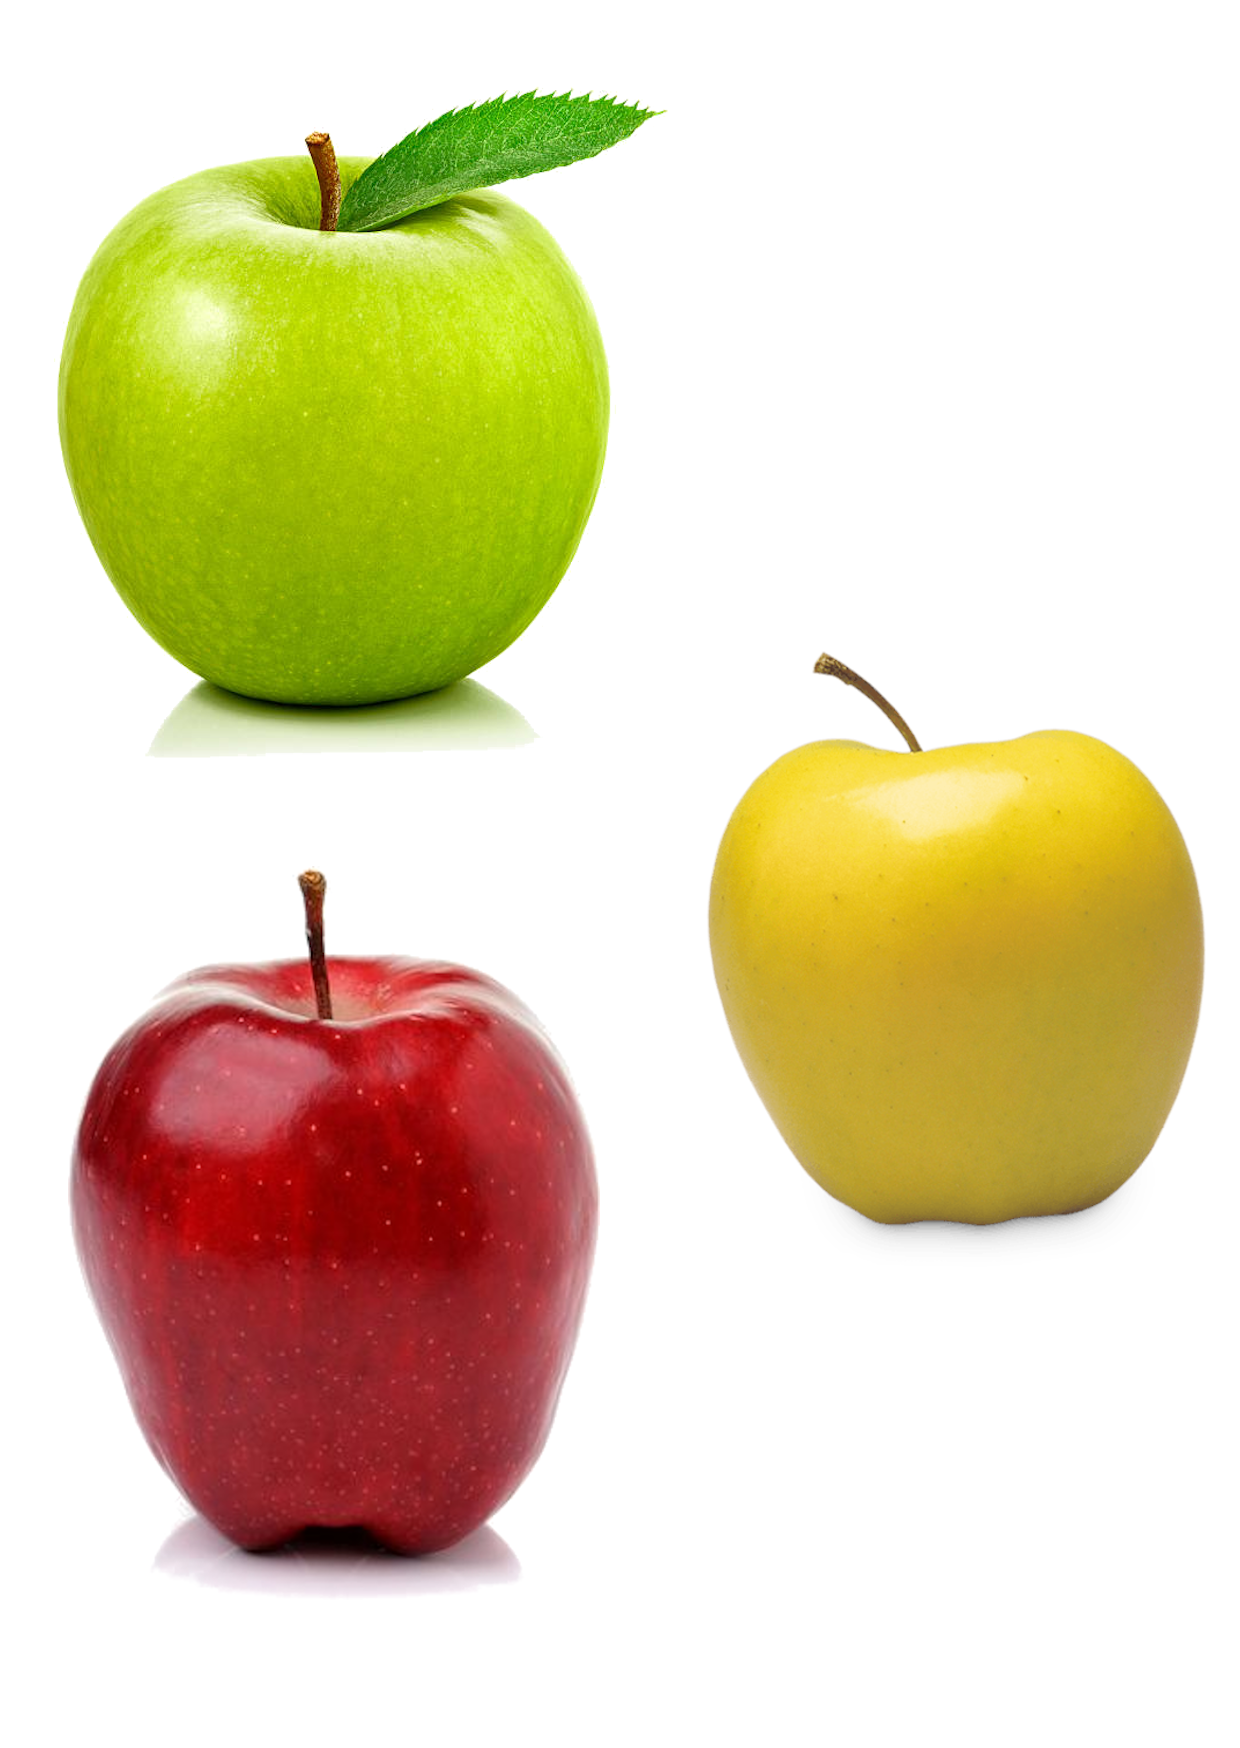
\includegraphics[width=0.3\textwidth]{3different.png}
	\end{figure}
	% TODO: some quantitative results

\end{frame}

\begin{frame}
	\frametitle{Named Entities and Wikification}
	% TODO
\end{frame}

\section{Classification: Legal \& Illegal Drugs, eBay}

\begin{frame}
	\frametitle{Models}
\end{frame}
\begin{frame}
	\frametitle{Manipulations}
	pos instead of
	dropped 
	...
\end{frame}

\begin{frame}
	\frametitle{legal DarkNet vs. eBay}
\end{frame}
\begin{frame}
	\frametitle{legal Drugs vs. illegal}
\end{frame}

\section{Cross-Domain Classification: Legal \& Illegal Forums}

\begin{frame}
	\frametitle{cross domain illegality}
	Forum: multi-topic\footnote{\textit{We assign Forum label to the multitopic forums unless the whole forum is related to
a single topic. e.g. a hacking forum was assigned
to Hacking class instead of Forum.}} \cite{AlNabki17}
\end{frame}

\section*{}

\begin{frame}
\frametitle{Conclusion}
\end{frame}

\begin{frame}[allowframebreaks]
\frametitle{References}
\bibliographystyle{apalike}
\tiny\bibliography{acl2019}
\end{frame}

\end{document}
